\section{问题一：数据质量评价、冲突消解与领域配比建模}
\label{sec:problem1}

\subsection{任务分解与整体口径}
\label{subsec:q1-framework}

问题一的三项任务共享同一批质量信号，输出对象却不同：质量评价须给出可跨样本比较、
可聚合到领域层的评分 $Q$；冲突分析须识别指标之间方向相反的张力并给出消解规则；
配比建模须建立 17 个配方域权重 $\boldsymbol{p}$ 与交叉熵损失的定量关系，
并论证是否以及如何引入 $Q$。三者若各用一套预处理，量表便无法拼接：领域级 $Q$ 是问题二的输入，
配比侧的损失须与问题三的成本口径对齐。本节先固定一套口径，再分别求解，
整体流程见图~\ref{fig:q1-framework}。质量主样本由 A1、A2、A3 拼合，共 272\,505 行；
19 行（18 行出自 A1、1 行出自 A3）有某个列表型字段整条缺失（该字段为 6 维向量，
如 ModernBERT 推理与专业性两列），不含质量信息，予以剔除，
保留 272\,486 行，占 99.993\%，与独立的缺失审计一致。22 个原始指标经规范化后合并为 20 列：
三个 DSIR 字段在逐 token 归一化后互相关仍高于 0.996，合并为一个代表量。
归一化以合并总体上的经验分位数为主口径，以按域分别归一化作为消融臂。
领域级聚合取 Huber $M$ 估计（稳健化参数 $k_{\mathrm{H}}=1.345$），区间由 $B_{\mathrm{boot}}=400$ 次自助重抽样给出，
并对聚合估计量、随机种子与扰动幅度分别作替换检验。

\begin{figure}[htbp]
  \centering
  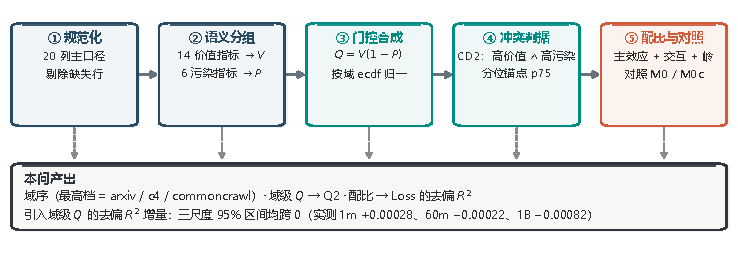
\includegraphics[width=0.98\linewidth]{figures/fig_framework_q1.pdf}
  \caption{问题一的方法流程。①—⑤ 为依次执行的五个环节：规范化（20 列主口径并剔除缺失行）、
  语义分组（14 个价值指标归入 $V$、6 个污染指标归入 $P$）、门控合成 $Q=V(1-P)$、
  冲突判据 CD2（高价值且高污染，分位数锚定）与配比建模（主效应加二阶交互，以岭回归正则化）。
  下方为本节交付物：领域序及其最高一档、领域级 $Q$（供问题二对照，其刻度对齐见问题二）、配比到损失的拟合优度，
  以及域级 $Q$ 增量在三尺度上的实测值与区间。}
  \label{fig:q1-framework}
\end{figure}

\subsection{22 个质量指标的方向统一与规范化}
\label{subsec:q1-direction}

22 个指标中，教育价值与整洁度等打分出自现代网页语料管线的判别器
\citep{penedo2024fineweb,warner2024modernbert}，其余为文本统计量与 DSIR 式对数似然比
\citep{xie2023dsir}；其方向并不一致，教育价值与流畅度越高越好，模板化重复与噪声占比越低越好。
赛题附录把方向标注指向《数据说明》，但该处可见文本中并无逐字段说明，方向表只能自行推得：
题面或原文明示者可核验，字段定义与指标间一致性支持者可推证，两者皆不足以判定者列为方向待定。
待定者恰为三个长度类字段（词数、句数与平均词长）。长度与质量的关系本不单调，过长与过短皆劣，
这与数据剪枝文献中样本统计量与有用性之间的非单调关系同源\citep{sorscher2022}，
而按区间而非固定阈值使用长度也是语料过滤的通行做法\citep{rae2021gopher}；
三项长度指标因此不取线性方向，而按到域内中位数的距离处理，两端受罚、中间得优。

DSIR 三列须单独讨论。原始字段是按 token 求和的对数似然比，属外延量，与长度高度绑定：
$\log(-\text{dsir})$ 与 $\log(\text{词数})$ 的 Pearson 相关为 0.937—0.939，
与词数的 Spearman 相关为 $-0.93$ 左右，直接用该字段排序几乎等同于按长度排序。
逐 token 归一化后，三个字段彼此的互相关升至 0.996 以上，名义上是三个域的相似度，
实际已高度接近同一构念，故合并为一个代表量。该处置同时修正了方向证据：
归一化前该字段与教育价值打分的 Spearman 为 $-0.499$，归一化后为 $+0.374$，
方向依据由建模判断升级为数据可证。

另一处长度纠缠落在一对统计量上：唯一词占比与一元词熵对 $\log(\text{词数})$ 的 Spearman
分别为 $-0.85$ 与 $+0.95$，方向相反。纯由长度即可生成约 $-0.81$ 的负相关；
把二者的长度分量各自剔除后，相关由 $-0.68$ 翻转为 $+0.92$，
可见原始负相关是长度诱导的伪矛盾，二者在同等长度下度量的是同一构念，即词汇多样性。
本节未施加校正，因为校正会同时制造冗余：残差化后二者相关为 $+0.92$，
在等权平均中近乎重复计入同一构念。

归一化取经验分位数，即以合并总体上的中位秩作单调映射（式~\eqref{eq:q1-ecdf}）：
\begin{equation}
  z_j(x)=\frac{R_j(x)+1/2}{n+1},\qquad
  R_j(x)=\tfrac{1}{2}\bigl(\#\{i:x_{ij}<x\}+\#\{i:x_{ij}\le x\}\bigr),
  \label{eq:q1-ecdf}
\end{equation}
$z_j\in(0,1)$ 且对单调变换不变。取分位数而非字面极差，是因若干字段量纲跨度极大，
例如 DSIR 原始值的中位数为 $-2.4\times10^{3}$、最小值为 $-2.0\times10^{6}$，
字面 Min--Max 会把几乎全部样本压进贴近 0 的窄带；对照实现为 1\%--99\% 截尾后的 Min--Max。
方向统一按式~\eqref{eq:q1-direction} 施加：
\begin{equation}
  u_j(x)=
  \begin{cases}
    z_j(x), & s_j=+1,\\
    1-z_j(x), & s_j=-1,\\
    1-2\,|z_j(x)-\tfrac{1}{2}|, & s_j=0,
  \end{cases}
  \label{eq:q1-direction}
\end{equation}
$s_j=0$ 即前述非单调的长度类指标。五个污染类指标（非字母词占比、最高频 2-gram 与 3-gram
字符占比、大写字母占比、数字字符占比）方向为负，统一取 $1-z_j$；
广告判别器的输出是两类对数几率之差 $\text{pos}_1-\text{pos}_0$，该差值本身已是「不像广告」，
方向为正，无须附加转换，其污染贡献在合成时取补。表~\ref{tab:q1-direction} 汇总 22 个原始指标的
分组、原始方向与统一方式。

\begin{table}[htbp]
  \centering
  \caption{22 个质量指标的方向统一与规范化处置。列数按原始字段计，DSIR 三列合并后主口径为 20 列；
  $V$、$P$ 为合成时的语义分组。}
  \label{tab:q1-direction}
  \begin{tabular}{@{}p{0.20\linewidth}p{0.30\linewidth}cp{0.30\linewidth}@{}}
    \toprule
    类别 & 指标 & 列数 & 统一方式 \\
    \midrule
    教育/专业度判别器 & 教育价值、质量评级、ModernBERT 四项（整洁度、可读性、推理、专业性）
      & 6 & 原始方向为正，直接取 $z_j$ \\
    广告与流畅度 & 广告性 margin、流畅度 margin & 2 & 差值本身即为「越高越好」，不附加转换 \\
    DSIR 相似度 & 三个域的对数似然比 & 3 & 先除以词数逐 token 归一化，再合并为一个代表量 \\
    长度类 & 词数、句数、平均词长 & 3 & 方向非单调，按 $1-2|z_j-\frac12|$ 处理 \\
    词汇多样性 & 唯一词占比、一元词熵 & 2 & 原始方向为正，取 $z_j$；不做长度校正 \\
    污染类 & 非字母词占比、2-gram 与 3-gram 字符占比、大写字母占比、数字字符占比
      & 5 & 原始方向为负，取 $1-z_j$ \\
    句子完整性 & 以终止标点结尾的行占比 & 1 & 原始方向为正，直接取 $z_j$ \\
    \bottomrule
  \end{tabular}
\end{table}

\subsection{门控合成与域级质量评分}
\label{subsec:q1-domain}

方向统一后，$V$ 组 14 列与 $P$ 组 6 列分别度量价值与污染。等权平均把两类信号置于同一尺度相抵：
模板化但通顺的推广文案可凭价值分抵消污染分，既不合语料治理的经验，也无法定义冲突。
本节改用门控合成：
\begin{equation}
  Q(x)=V(x)\,\bigl[1-P(x)\bigr],\qquad
  V(x)=\frac{1}{|V|}\sum_{j\in V}u_j(x),\qquad
  P(x)=\frac{1}{|P|}\sum_{j\in P}\bigl[1-u_j(x)\bigr].
  \label{eq:q1-gate}
\end{equation}
式~\eqref{eq:q1-gate} 中 $P$ 落在 $(0,1)$ 内，故 $Q\in(0,1)$ 且无须截断，与问题三中 $g(Q)=5\times10^{9}Q^{4}$
一类在非负区间单调的定义相容。分组依据是字段语义而非相关结构：组内平均相关 0.150 与 0.026、
组间 $-0.013$，三者同量级，不能声称其由相关结构导出，这一点在分组扰动检验中会再次出现。

领域级 $Q$ 由域内样本聚合。逐域分布右偏且含少量离群文档，算术均值会被尾部拉动，
本节取 Huber $M$ 估计
\begin{equation}
  \hat Q_d=\arg\min_{m}\sum_{x\in d}\rho_{k_{\mathrm{H}}}\!\left(\frac{Q(x)-m}{\hat\sigma_d}\right),
  \qquad
  \rho_{k_{\mathrm{H}}}(r)=
  \begin{cases}
    r^{2}/2, & |r|\le k_{\mathrm{H}},\\
    k_{\mathrm{H}}|r|-k_{\mathrm{H}}^{2}/2, & |r|>k_{\mathrm{H}},
  \end{cases}
  \label{eq:q1-huber}
\end{equation}
式~\eqref{eq:q1-huber} 中 $k_{\mathrm{H}}=1.345$，$\hat\sigma_d$ 由中位绝对偏差按 1.4826 折算，区间由 $B_{\mathrm{boot}}=400$ 次自助重抽样给出。
表~\ref{tab:q1-domain-quality} 同表列出等权平均基线 $M_0$ 与门控合成 $M_1$ 的域级取值与区间。

\begin{table}[htbp]
  \centering
  \caption{七个领域的质量评分 $Q$ 与 95\% 自助区间（$B_{\mathrm{boot}}=400$，Huber $M$ 估计，合并总体分位数口径）。
  $n$ 为域内样本量。表中数值保留四位小数，与自助样本的蒙特卡洛精度相称。}
  \label{tab:q1-domain-quality}
  \begin{tabular}{@{}lccccc@{}}
    \toprule
    领域 & $n$ & $M_0$ 等权平均 & $M_0$ 区间 & $M_1$ 门控合成 & $M_1$ 区间 \\
    \midrule
    arxiv        & 18\,942  & 0.6494 & (0.6490, 0.6498) & 0.3815 & (0.3807, 0.3823) \\
    c4           & 10\,000  & 0.6019 & (0.6000, 0.6036) & 0.3638 & (0.3619, 0.3658) \\
    commoncrawl  & 9\,636   & 0.6013 & (0.5999, 0.6027) & 0.3479 & (0.3464, 0.3498) \\
    stackexchange & 10\,000 & 0.5830 & (0.5819, 0.5842) & 0.2943 & (0.2929, 0.2958) \\
    wikipedia    & 9\,986   & 0.5326 & (0.5310, 0.5343) & 0.2556 & (0.2542, 0.2572) \\
    book         & 171      & 0.5264 & (0.5170, 0.5356) & 0.2668 & (0.2584, 0.2753) \\
    github       & 213\,751 & 0.4736 & (0.4733, 0.4740) & 0.2233 & (0.2230, 0.2236) \\
    \bottomrule
  \end{tabular}
\end{table}

图~\ref{fig:q1-gating-stability} 给出预先声明的两项判据。等权平均在 21 个域对中分辨出 19 对，
门控合成分辨出全部 21 对，新增的两对正是 book 与 wikipedia、c4 与 commoncrawl。
40 次 $\pm10\%$ 列权重扰动下，门控合成的域序 Kendall $\tau$ 均值为 0.9976、
域序完全不变的重复比为 0.975，等权平均为 0.9595 与 0.625，两者之差的 95\% 区间
$[0.019,0.057]$ 不含零；放宽到 $\pm20\%$ 差值仍为 $+0.0500$（$[0.0262,0.0762]$），
$\pm30\%$ 为 $+0.0357$（$[0.0023,0.0714]$），该档已超出小扰动的合理范围，仅作探索性报告。

\begin{figure}[htbp]
  \centering
  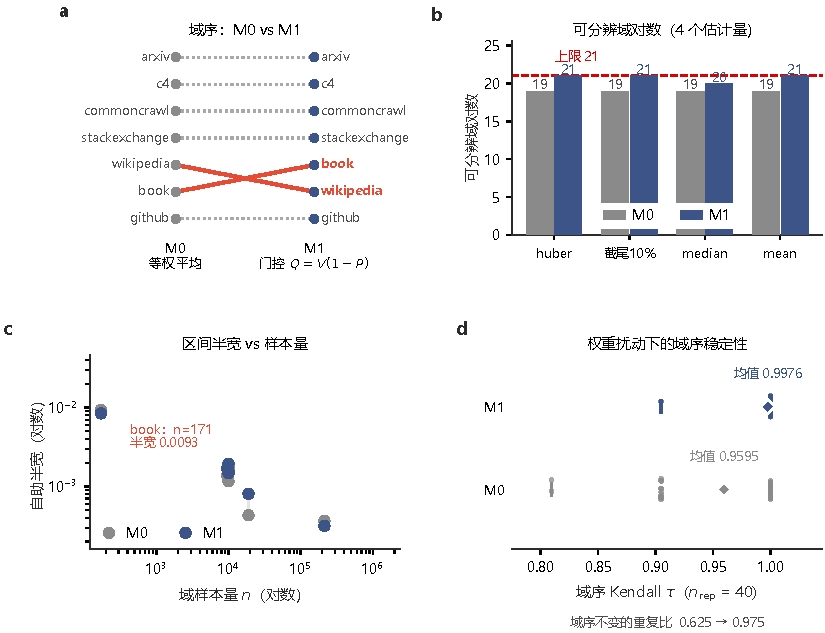
\includegraphics[width=0.98\linewidth]{figures/fig_q1_gating_stability.pdf}
  \caption{门控合成与等权平均的对照。(a) 两法的领域序，虚线为次序不变，红色横线标出唯一互换的一对；
  (b) 四个聚合估计量下的可分辨域对数，虚线为上限 21；(c) 域级自助半宽对域样本量（双对数），
  左下角孤点为 book（$n=171$，半宽 0.0093）；(d) 40 次权重扰动下的域序 Kendall $\tau$ 分布，
  门控合成均值 0.9976、等权平均 0.9595，域序不变的重复比自 0.625 升至 0.975。}
  \label{fig:q1-gating-stability}
\end{figure}

域序须谨慎表述。合并总体口径下的门控合成给出
$\text{arxiv}>c4>\text{commoncrawl}>\text{stackexchange}>\text{book}>\text{wikipedia}>\text{github}$，
等权平均仅在 book 与 wikipedia 处与之相反。该次序与直觉不完全吻合，其中一部分应是真实的：
22 个指标大多是面向现代网页文本训练的判别器，book 域的 171 条样本取自 Gutenberg 公版书，
其拼写与排版在现代可读性打分上本就吃亏，该偏差不应通过调方向消除，而应作为口径限制保留。
可断言的结论有三处。其一，最高一档恒为
$\{\text{arxiv},\text{c4},\text{commoncrawl}\}$，在基线与 8 个分组扰动变体共 9 个配置下不变；
但 arxiv 居该档之首并不稳固：把污染组中任一列移入价值组后，其档内位次实测取到过 1、2、3，
其中两个变体下 c4 的反超裕度达 9.38 倍与 3.92 倍区间半宽和，属统计可分。
机理在于 $Q=V(1-P)$ 中同一列置于 $V$ 是加性贡献、置于 $P$ 是乘性门控，归属变更即改变其
函数角色，而分组是纯语义划分；故本节只报最高一档，不对档内位次作断言。其二，c4 优于
commoncrawl（裕度 4.37 倍区间半宽和）与 github 居末在基线与全部变体下成立，方向可照常报告。
其三，book 与 wikipedia 统计上不可区分：域级 $Q$ 差在等权平均下为 0.00617（wikipedia 略高）、
在门控合成下为 0.01113（book 略高），方向随合成方式反转，较大一侧的裕度仅为区间半宽和的
1.12 倍。book 域区间偏宽可由样本量解释：等 $n$ 对照重抽给出的半宽为 0.00880，
与表~\ref{tab:q1-domain-quality} 中门控合成的自助区间同量级但不同源，是 github 的 25 倍以上；
把其余六域各自无放回降采样到 $n=171$ 并重复 40 次，半宽包络为 $[0.00715,0.01691]$，
book 的实测半宽落在包络内且偏窄端，无须归因于域内异质。该域级 $Q$ 供问题二使用时须附说明：
book 的取值不可靠，下游环节须为其设置敏感性臂。

一项限制在此处即可确证：用 $Q$ 区分 arxiv 与 github 的 AUC 在门控合成下为 0.9486、
等权平均下为 0.9741，即单一标量评分高度可由领域标签还原。这一缺陷并非本规格引入：
数据阶段已查明 25 个候选标量中有 15 个近乎完美地分离 arxiv 与 github，
全部 22 个指标的最大域对分离度均不低于 0.30。按域归一化虽能把该 AUC 压到 0.50 附近，
但域级 $Q$ 同时近乎恒等（域间极差由 0.1582 降至 0.0115）、21 个域对中仅 9 对可分辨，
故它只是消融臂，用以量化主口径选择的代价。在这批指标上，
单一标量评分不可能同时做到跨域可比与域去混淆。

\subsection{质量冲突的定义与消解}
\label{subsec:q1-conflict}

冲突在门控形式下有自然的含义：同一篇文本在价值与污染两类指标上同时取高分，
即一端被判为有用，另一端被判为模板化。绝对阈值不适合描述这种现象：把两维阈值都定在 0.75，
实测冲突率恰为零，因为两维各自的 75\% 分位点都低于该值。本节改以分位数锚定，主判据取
式~\eqref{eq:q1-cd2}：
\begin{equation}
  \text{CD2}:\quad x\ \text{为冲突}\iff V(x)>Q_{0.75}(V)\ \text{且}\ P(x)>Q_{0.75}(P),
  \label{eq:q1-cd2}
\end{equation}
即在两维上同时落入上四分位。冲突率对锚点单调，$p_{70}$、$p_{75}$、$p_{80}$ 三档分别为
0.0687、0.0408、0.0208，主报值 0.0408 落在 $(0.01,0.50)$ 内，既非退化也非饱和。
消解规则相应地不是删除而是标注：冲突样本保留在样本集中，但在涉及质量提升的
成本口径中宜按质量上界处理。本文未对冲突比例另设敏感臂，该处置只作口径声明。

作为对照的另三个判据基于组内指标的异常度，而非两维之间的张力。表~\ref{tab:q1-conflict}
上半部分给出四判据在三档锚点下的全局冲突率。MAD 锚定判据的全局率恰等于 $1$ 减去锚点
（实测 0.3000、0.2500、0.2000），这是「一维离散度取分位数阈值」的恒等式，不含样本信息，
故该判据只报告域级分布与子集重叠度；「至少三高且至少三低」判据在 $p_{70}$ 下给出 0.8357，
把绝大多数样本判为冲突，同样退化。按 $p_{75}$ 锚点衡量，主判据与其余三者所标识的冲突子集
重叠度很低，Jaccard 系数为 0.030、0.036 与 0.045，而两个异常度判据彼此重叠到 0.512，
实质是同一子集的不同切法。

\begin{table}[htbp]
  \centering
  \caption{冲突判据的锚点敏感性（上半，合并总体口径的全局冲突率）与主判据的域级冲突率
  （下半，合并总体口径；$p_{75}$ 锚点下取 CD2 与「至少三高且至少三低」两者，
  第二列取 CD1 在固定参考阈 0.25 处的衔接对照版，其取值与锚点无关）。
  上半部分末行为「至少三高且至少三低」判据，在 $p_{70}$ 下已把 83.57\% 的样本判为冲突；
  下半部分用以显示异常度判据的域级退化。}
  \label{tab:q1-conflict}
  \begin{tabular}{@{}lccc@{}}
    \toprule
    \multicolumn{4}{@{}l}{\emph{(a) 全局冲突率对锚点的响应}}\\
    \midrule
    判据 & $p_{70}$ & $p_{75}$ & $p_{80}$ \\
    \midrule
    CD2 高价值且高污染（主判据） & 0.0687 & \textbf{0.0408} & 0.0208 \\
    MAD 锚定（一维离散度） & 0.3000 & 0.2500 & 0.2000 \\
    至少五高且至少五低 & 0.3951 & 0.2181 & 0.1152 \\
    至少三高且至少三低 & 0.8357 & 0.6561 & 0.4688 \\
    \midrule
    \multicolumn{4}{@{}l}{\emph{(b) $p_{75}$ 锚点下的域级冲突率}}\\
    \midrule
    领域 & CD2 & CD1 固定阈 0.25 & 至少三高且至少三低 \\
    \midrule
    stackexchange & 0.174 & 0.210 & 0.608 \\
    wikipedia     & 0.090 & 0.542 & 0.878 \\
    arxiv         & 0.038 & 0.878 & 0.958 \\
    github        & 0.036 & 0.209 & 0.606 \\
    book          & 0.035 & 0.994 & 1.000 \\
    commoncrawl   & 0.013 & 0.653 & 0.820 \\
    c4            & 0.004 & 0.731 & 0.822 \\
    \bottomrule
  \end{tabular}
\end{table}

主判据的域级取值给出本节最有信息量的一条读数：stackexchange 的冲突率为 0.174，
c4 为 0.004，两者相差 43 倍，book 为 0.035 处于低位；两个异常度判据恰在此处失效，
它们把 book 域几乎全部判为冲突（CD1 固定阈 0.25 下 0.994，另一判据下 1.000），
即 171 条公版书全部进入冲突集，与该域的质量表现明显不符。
图~\ref{fig:q1-conflict-matrix} 以热力图给出四判据在两档归一化口径下的完整取值。
冲突子集相对全体均值，在可读性、质量评级与整洁度上分别高出 0.263、0.244 与 0.241，
在数字字符占比、大写字母占比与最高频 3-gram 字符占比上分别低出 0.198、0.191 与 0.182，
广告性 margin 与 2-gram 占比各低 0.122，即这批样本写得规整通顺而模板化程度偏低，
与判据的设计意图一致，逐条样本已连同其在原文件中的位置落盘。
分组扰动下主判据的冲突率在 0.0236 至 0.0568 之间变动，消融臂给出 0.0550，
可见其量级不依赖分组细节，这与域序头名依赖分组细节形成对照。

\begin{figure}[htbp]
  \centering
  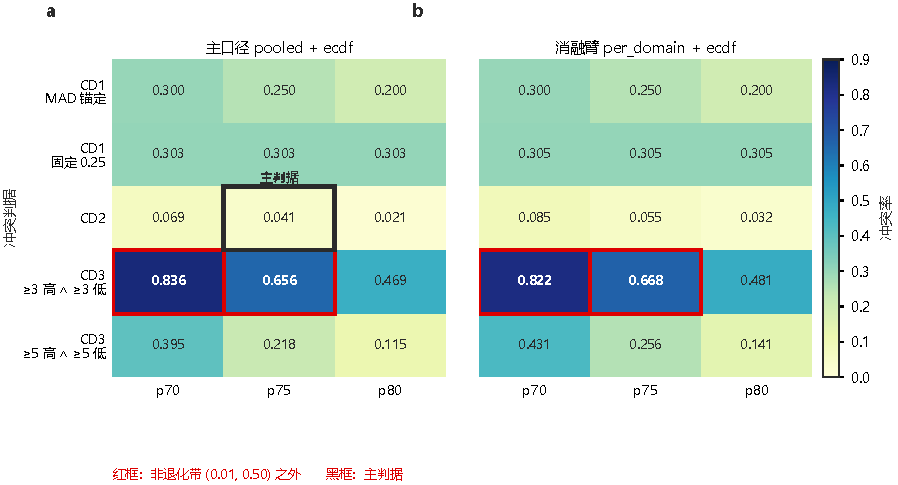
\includegraphics[width=0.98\linewidth]{figures/fig_q1_conflict_matrix.pdf}
  \caption{四判据与三档锚点下的全局冲突率热力图，横轴为锚点分位数 $p_{70}$、$p_{75}$、$p_{80}$，
  纵轴为判据，色标为冲突率。(a) 合并总体口径，(b) 按域归一化的消融臂。
  黑框标出主判据 CD2 在 $p_{75}$ 处的取值 0.041，红框标出取值越出非退化带 $(0.01,0.50)$ 的格子；
  两档口径下越界的格子相同，均为「至少三高且至少三低」判据在 $p_{70}$ 处的 0.836 与 0.822。}
  \label{fig:q1-conflict-matrix}
\end{figure}

\subsection{配比建模与质量评分的增量检验}
\label{subsec:q1-mixture}

配比侧要建立 17 个配方域权重与交叉熵损失之间的关系。17 个域取自 Pile 的域划分\citep{gao2020pile}，
配比行满足单纯形约束；自变量中位数上约有半数取精确零，对数比变换不可用，故直接以配比作自变量。
基线模型对 13 个可观测损失域拟合式~\eqref{eq:q1-mixture} 的去截距线性形式，
扩展模型在其上加入全部二阶交互项
$p_dp_{d'}$（共 153 个特征）并以岭回归正则化，正则强度取交叉验证选定的 $10^{-3}$，
两个模型分别记为 $M_{0c}$ 与 $M_{1c}$。
\begin{equation}
  \widehat{L}=\sum_{d\in\mathcal{D}}p_d\,\theta_d,\qquad
  \sum_{d\in\mathcal{D}}p_d=1,
  \label{eq:q1-mixture}
\end{equation}
去截距是必要的：截距与单纯形约束共同造成设计矩阵近乎奇异，含截距时的条件数为 4773，
去截距后降至 61。配比小样本回归已有先例\citep{liu2024regmix}，领域权重亦可在训练中动态调整
\citep{xie2023doremi}；本节取其静态估计，以便把系数作为可解释的域效应。

跨尺度验证须先澄清口径。原始 $R^{2}$ 在 1m 尺度为 0.913，到 60m 与 1B 却分别为
$-8.412$ 与 $-173.115$：偏差占均方根误差的 98.8\% 与 99.9\%，误差几乎全部来自损失量级
随规模的平移，而非拟合失效。去掉按尺度估计的常数偏移后，$R^{2}$ 回到 0.771 与 0.705，
秩相关为 0.922 与 0.887。即配比到损失的形状跨尺度可迁移，只有水平随规模平移，
故验证一律报告去偏 $R^{2}$ 与秩相关，原始 $R^{2}$ 不作单独引用。在去偏口径下，
$M_{1c}$ 的增益只在 1m 尺度为正（$+0.0703$），60m 为 $-0.0050$、1B 为 $-0.0464$，
秩相关增益亦为负，不构成跨尺度优势；本节因此以 $M_{0c}$ 为主模型，
$M_{1c}$ 仅作组合效应的辅助证据。$M_{0c}$ 的 17 个主效应系数在自助重抽样下符号全部稳定，
平均相对标准误 0.034；$M_{1c}$ 的 153 个特征中符号稳定率不低于 0.95 的只有 84 个，
含主效应 17 个全部稳定与交互项 67 个稳定（其中不低于 0.99 的 53 个），其余 69 项不予报告。
稳定子集之外的单个交互系数不得解释为领域之间的替代或互补，子集之内也只支持方向性陈述
而非定量替代率：正则强度增减一个数量级时稳定子集大小在 80 与 125 之间变动，
逐项解释因此不可靠。

目标口径本身需要声明。主目标以配比加权各域的损失，配比同时出现在等式两侧，存在部分循环；
本节仍以其为主口径，是其训练 $R^{2}$（0.8958）远高于简单平均口径（0.2962），
后者自身不是可主报的口径（1B 去偏 $R^{2}$ 为 $-8.667$），只作方向对照。
两个口径下域效应的量级排序实质相反，系数向量的 Spearman 相关为 $-0.5809$，
故下文关于域效应量级的排序均以加权目标口径为前提。

质量评分是否应引入配比模型，由一次嵌套检验回答：在 17 维配比之上加入域级 $Q$ 按配比加权
得到的语料质量项，比较同一子集上的去偏 $R^{2}$。表~\ref{tab:q1-mixture} 下半部分与
图~\ref{fig:q1-q-increment}(b) 给出结果，三个尺度的增量为 $+0.00028$、$-0.00022$、$-0.00082$，
95\% 区间均含零，无可检出的增量。
成因是构造性的：$Q_{\text{corpus}}$ 本身是 $\boldsymbol{p}$ 的函数，17 个配方域中只有 6 个
能对应到质量域，映射域的配比质量中位数仅 0.5995；512 个训练行中 5 行在映射域上配比质量全为零，
已剔除，两个模型在其余 507 行上拟合与评估，条件数由 60.98 升至 86.07。
向一个已含 $\boldsymbol{p}$ 的模型再放进 $\boldsymbol{p}$ 的函数，增量无从产生。
判定条件须一并给出：1B 尺度只有 64 个观测，其增量上界仅 $+1.5\times10^{-5}$，
与自助重抽样的蒙特卡洛波动同量级；把该格的自助次数提高后，$B_{\mathrm{boot}}=4000$ 与 $B_{\mathrm{boot}}=40000$
各跨 8 个独立种子均一致给出含零的区间，而 $B_{\mathrm{boot}}=400$ 下上界极差为 $1.40\times10^{-4}$，
高于上界离零的距离约 $5\times10^{-5}$。故「三尺度区间均含零」成立，
条件是 $B\ge4000$ 且 $n=64$；四个不同质量来源的同类检验中，
12 个「来源 $\times$ 尺度」格子有 11 个区间含零。

\begin{table}[htbp]
  \centering
  \caption{配比模型的跨尺度验证与质量评分的增量检验。上半部分为两个模型在三个尺度上的
  去尺度偏移 $R^{2}$、秩相关，以及基线模型的原始 $R^{2}$ 与偏差占均方根误差之比；
  下半部分为在 17 维配比之上引入域级 $Q$ 后的去偏 $R^{2}$ 与增量区间（$B_{\mathrm{boot}}=400$，
  「仅 $p$」与「$p+Q$」在同一 507 行子集上拟合与评估）。增量与区间端点保留五位小数，
  1B 尺度区间改以科学计数法书写以保留其有效数字。}
  \label{tab:q1-mixture}
  \begin{tabular}{@{}lcccccc@{}}
    \toprule
    \multicolumn{7}{@{}l}{\emph{(a) 跨尺度验证（$R^{2}$ 已去尺度偏移）}}\\
    \midrule
    尺度 & $M_{0c}$ $R^{2}$ & $M_{1c}$ $R^{2}$ & $R^{2}$ 增益 & $M_{0c}$ 秩相关 & $M_{1c}$ 秩相关
      & 原始 $R^{2}$ / 偏差占比 \\
    \midrule
    1m   & 0.9131 & 0.9834 & $+0.0703$ & 0.9531 & 0.9903 & 0.9130 / 0.035 \\
    60m  & 0.7706 & 0.7656 & $-0.0050$ & 0.9221 & 0.9018 & $-8.412$ / 0.988 \\
    1B   & 0.7047 & 0.6583 & $-0.0464$ & 0.8872 & 0.8488 & $-173.115$ / 0.999 \\
    \midrule
    \multicolumn{7}{@{}l}{\emph{(b) 引入域级 $Q$ 的增量检验}}\\
    \midrule
    尺度 & 仅 $p$ & $p+Q$ & 增量 & \multicolumn{2}{c}{95\% 区间} & 显著 \\
    \midrule
    1m   & 0.9129 & 0.9132 & $+0.00028$ & $(-0.00022,$ & $+0.00080)$ & 否 \\
    60m  & 0.7716 & 0.7714 & $-0.00022$ & $(-0.00066,$ & $+0.00013)$ & 否 \\
    1B   & 0.7075 & 0.7067 & $-0.00082$ & $(-2.06\times10^{-3},$ & $+1.5\times10^{-5})$ & 否 \\
    \bottomrule
  \end{tabular}
\end{table}

\begin{figure}[htbp]
  \centering
  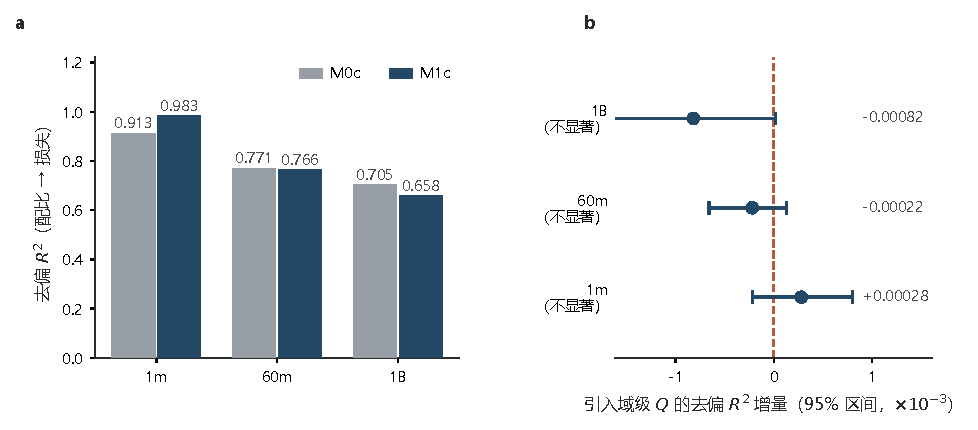
\includegraphics[width=0.98\linewidth]{figures/fig_q1_q_increment.pdf}
  \caption{配比模型的跨尺度表现与质量评分的增量。(a) 三个尺度上两模型的去尺度偏移 $R^{2}$，
  1m 尺度上二阶交互模型 0.983 高于线性模型 0.913，60m 与 1B 两尺度上两者互有高低；
  (b) 引入域级 $Q$ 后去偏 $R^{2}$ 的增量与 95\% 自助区间，三条区间均跨过零线（虚线），
  1B 尺度的上界仅 $+1.5\times10^{-5}$。}
  \label{fig:q1-q-increment}
\end{figure}

\subsection{局限与适用范围}
\label{subsec:q1-limits}

方向表不是数据自带的信息：《数据说明》未给出 22 个指标的方向标注，该表由本节依据字段定义、
指标间一致性与原文抽样推得，并按可信度分层（证据可直接核验者 8 项、
由字段定义与指标间一致性推证者 11 项、方向待定者 3 项）；待定的三项恰为长度类指标，
凡以该三项为承重项的读数都以本节的裁定为前提，并另报方向替换下的敏感性。
A18 的文本统计量由本节自行计算，与 A1--A3 中数据集自带的模型打分不同源，
两者只能作趋势与秩一致性的对照，绝对值不可比。

质量侧的结论各有边界。领域序的最高一档 $\{\text{arxiv},\text{c4},\text{commoncrawl}\}$、
c4 优于 commoncrawl 与 github 居末在基线与分组扰动下均成立；arxiv 是否居首依赖 $V/P$ 分组中
个别列的单列归属，本节不作断言。book 域的 171 条样本使该域的域级 $Q$ 带有宽区间，
下游使用须附敏感性。单一标量评分无法同时做到跨域可比与域去混淆，是这批指标的性质所决定的
可证限制，而非本节规格的缺欠；主口径 $Q$ 与 $\log\text{词数}$ 的 Spearman 相关为 0.499，
即该标量本身仍带长度暴露，跨域可比同样受各域长度分布约束。相应地，本文对领域间的质量比较
只在最高一档的集合层面作出，稳定子集之外交互系数不作解释，域效应的量级排序以配比加权
目标口径为前提。

配比侧的读数是样本条件的结果：训练行只有 512 行，损失域只有 13 个，
153 个二阶交互特征在该样本量下大部分不可辨识，增益集中于最小尺度也就不难理解。
A12--A15 为外推表或训练集子集；其中外推表（A12、A14）的配比行与训练集的重叠率为 1.0，
只能检验损失的外推而不能检验配比的泛化，故本节未用它们支持任何定量结论。质量评分的
增量检验为零结果，成因是质量项与配比的构造性相关，而非质量信息无用；
在本数据条件下，该检验无法把
「质量是否有用」与「质量项能否在已含配比的模型中被辨识」分开。三项稳健性检验的结果性质不同：
分组扰动是一项真发现，它使领域序的表述被收窄；1B 尺度的增量检验反映自助次数不足，
该格在 $B_{\mathrm{boot}}=400$ 下不可判定；目标口径替换检验则判据设计失效，其预声明判据为两口径下系数符号
的一致率，而目标取损失、设计矩阵去截距且配比之和为一，每个系数即该域的损失水平，
17 个系数必然同号，一致率 1.000 是平凡结果，不构成证据；该检验真正提供信息的是系数向量的
排序反转（Spearman $-0.5809$），它支持的是一条限制，即域效应的量级排序依赖目标口径。
